\documentclass[11pt,letterpaper]{article}
\usepackage[utf8]{inputenc}
\usepackage[sc]{mathpazo}

\usepackage[T1]{fontenc}
\usepackage{amsmath}
\usepackage{amsfonts}
\usepackage{amssymb}
\usepackage{graphicx}
\usepackage{comment}
\usepackage{bbm}
\usepackage{hyperref}
\usepackage{apacite}
\usepackage{natbib}
\usepackage{har2nat}
\usepackage[width=16.00cm, height=23.00cm]{geometry}
\usepackage{tablefootnote}
\usepackage{multirow}
\usepackage{longtable}
\usepackage{rotating, tabularx}
\usepackage{booktabs}
\usepackage{threeparttable}
\usepackage[table,xcdraw]{xcolor}
\usepackage[dvips]{xcolor}
\usepackage{pdflscape, lipsum}
\usepackage{tabularx}
\usepackage{url}
\usepackage{float}
\usepackage[capposition=top]{floatrow}
\usepackage{subcaption}

\usepackage{xr}
\externaldocument{MPHI}
\usepackage[toc,page]{appendix}

\definecolorseries

\usepackage[pagewise]{lineno}
%\linenumbers

\renewcommand{\baselinestretch}{1.3}
%\linespread{1.3}         % Palladio needs more leading (space between lines)


\hypersetup{colorlinks,linkcolor={[rgb]0.7, 0.11, 0.11},citecolor={[rgb]0.7, 0.11, 0.11}, filecolor={[rgb]0.7, 0.11, 0.11}, urlcolor={[rgb]0.7, 0.11, 0.11}}  
%magenta
%\hypersetup{colorlinks=false, urlbordercolor=blue}
%0,0.88502,1,0
\usepackage{booktabs,siunitx,amsmath,caption}

%-------------------------------------------------------------------
\begin{document}
	
\title{\textbf{Monetary Policy and Household Income Distribution: An Empirical Analysis from Cambodia \\
						Online Appendix}}
\author{Kosal Nith \\
						\small{Future Forum}  
						%\and
						%Thounimith Phay  \\
						%\small{Royal School of Administration}  
					}
%-------------------------------------------------------------------	  
\maketitle
\appendix 
%	\part*{Appendix}\label{app:dix}
	\pagenumbering{Arabic}
	\renewcommand*{\thepage}{A\arabic{page}}
	\numberwithin{equation}{section}
	\renewcommand{\thetable}{A\arabic{table}}
	\renewcommand{\thefigure}{A\arabic{figure}}	
	
	\vspace{-3em}
	
\tableofcontents	

%-------------------------------------------------------------------	  
\section{Data Appendix}\label{app:b}
%-------------------------------------------------------------------	
In this section, I deliver additional tables of summary statistics for macro data and microdata used as monetary policy shocks, macroeconomic and financial aggregates, and household wealth through three monetary policy channels. First, I present macro data, and then I give detailed statistics on the level of households. Finally, I show the histogram of the distribution of household wealth across the country and the region. 

%-------------------------------------------------------------------	  
	\subsection{Macro Data}\label{app:b1}
%-------------------------------------------------------------------  
This section offers the descriptive statistics of macroeconomic aggregates used as monetary policy shocks in section \ref{sec:r2}. There are five main variables: inflation, output, unemployment rate, interest rate, exchange rate, and broad money. 

		\begin{table}[H]
	\centering
	\caption{Summary statistics for macroeconomic variables}
	\label{app:tabm1}
	\resizebox{.95\textwidth}{!}{%
		\begin{tabular}{@{}lccccccc@{}} 
			\hline \hline
			&       Obs.&        Mean&          S.D.&         Min.&         Max. & Unit& Source\\
			\hline
			Inflation         &          46&        3.01&        1.51&        0.70&        7.06 & Percent& NIS\\
			Output      &          46&        4.83&        1.39&        2.78&        7.45 & Billion dollars &NIS\\
			Unemployment rates       &          46&        0.43&        0.23&        0.13&        0.77 & Percent& ILO\\
			Interest rates       &          46&        5.26&        0.77&        4.19&        6.91 &Weighted average rate&NBC\\
			Exchange rates     &          46&     4071.58&       52.64&     3985.60&     4257.36 &Khmer riels/US dollars& NBC\\
			M2         &          46&       15.66&        9.84&        4.13&       36.29 &Billion dollars&NBC\\

			\hline\hline
		\end{tabular}%
	}
	\begin{tablenotes}
	\footnotesize
	\item \textbf{Note:} This table displays the descriptive statistics of macroeconomic variables that using for the investigation of monetary policy shocks. The second column reports the number of observations, the third presents the mean, and the fourth column is standard deviation errors. Many variables are observed quarterly, and some variables, such as the unemployment rate and output, are recorded annually. I suppose the real input growth and the employment rate have the same proposition every quarter in a whole year, and then I multiply it with 4 to get the quarter data. The dataset comes from the National Institute of Statistics, the International Labor Organization, and the National Bank of Cambodia.       

	\end{tablenotes} 
	
\end{table}    	


\subsection{Summary Statistics of Micro Data}\label{app:tabdata}
This part presents the descriptive statistics of household data from the 2014--2019/2020. I classified four main wealth channels: income, consumption, assets and liabilities. According to the questionnaire, I get the wealth data and household demographics as follow:  
\vspace{1.5em}

\noindent \textbf{Income.} Household income  = wages + non agricultural income + crops income + other crops income + rice income + seed income + livestock income + fishery income + pond rent income + forestary income + land sold income + building rend income + other incomes. 
\vspace{1em}

\noindent \textbf{Consumption.} Household consumption expenditure = food and non food expenditure + durable goods expenditure = food consumption + housing consumption + dwelling repair spending + building spending + house rent consumption + livestock consumption + forestry consumption + illness consumption, taxes expenditure + durable goods + land buying + land rent spending + education expenditure. 

\vspace{1em}

\noindent \textbf{Assets.} Household assets = non agricultural investment + rice stock + livestock stock + crops investment + livestock investment + fishery investment + forestry investment.

\vspace{1em}

\noindent \textbf{Liabilities.} Household liabilities = borrowing for agriculture activities + non agricultural activities + consumption needs + illness, injury, accident + emergency expenditure + rituals + dwelling improvement + durable goods + serving, existing debt + others. 

\vspace{1em}
\noindent The value of household wealth is calculated  in the annual by using the annual exchange rate of each year between Khmer riels and US dollars. There are about 4,038 riels per \$1 unit in 2014, 4,045 riels per \$1 unit in 2017 and 4,052 riels per \$1 in 2019. More wealth data are reported in monthly, therefore I multiply it with 12 to get the annually data. 
%-------------------------------------------------------------------  
\begin{table}[H]
	\centering
	\caption{Summary statistics for macroeconomic variables}
	\label{app:tabm1}
	\resizebox{.95\textwidth}{!}{%
		\begin{tabular}{@{}lccccccc@{}} 
			\hline \hline
			&       Obs.&        Mean&          S.D.&         Min.&         Max. & Unit& Source\\
			\hline
			Inflation         &          46&        3.01&        1.51&        0.70&        7.06 & Percent& NIS\\
			Output      &          46&        4.83&        1.39&        2.78&        7.45 & Billion dollars &NIS\\
			Unemployment rates       &          46&        0.43&        0.23&        0.13&        0.77 & Percent& ILO\\
			Interest rates       &          46&        5.26&        0.77&        4.19&        6.91 &Weighted average rate&NBC\\
			Exchange rates     &          46&     4071.58&       52.64&     3985.60&     4257.36 &Khmer riels/US dollars& NBC\\
			M2         &          46&       15.66&        9.84&        4.13&       36.29 &Billion dollars&NBC\\

			\hline\hline
		\end{tabular}%
	}
	\begin{tablenotes}
	\footnotesize
	\item \textbf{Note:} This table displays the descriptive statistics of macroeconomic variables that using for the investigation of monetary policy shocks. The second column reports the number of observations, the third presents the mean, and the fourth column is standard deviation errors. Many variables are observed quarterly, and some variables, such as the unemployment rate and output, are recorded annually. I suppose the real input growth and the employment rate have the same proposition every quarter in a whole year, and then I multiply it with 4 to get the quarter data. The dataset comes from the National Institute of Statistics, the International Labor Organization, and the National Bank of Cambodia.       

	\end{tablenotes} 
	
\end{table}    
\begin{table}[H]
	\centering
	\caption{Summary statistics for macroeconomic variables}
	\label{app:tabm1}
	\resizebox{.95\textwidth}{!}{%
		\begin{tabular}{@{}lccccccc@{}} 
			\hline \hline
			&       Obs.&        Mean&          S.D.&         Min.&         Max. & Unit& Source\\
			\hline
			Inflation         &          46&        3.01&        1.51&        0.70&        7.06 & Percent& NIS\\
			Output      &          46&        4.83&        1.39&        2.78&        7.45 & Billion dollars &NIS\\
			Unemployment rates       &          46&        0.43&        0.23&        0.13&        0.77 & Percent& ILO\\
			Interest rates       &          46&        5.26&        0.77&        4.19&        6.91 &Weighted average rate&NBC\\
			Exchange rates     &          46&     4071.58&       52.64&     3985.60&     4257.36 &Khmer riels/US dollars& NBC\\
			M2         &          46&       15.66&        9.84&        4.13&       36.29 &Billion dollars&NBC\\

			\hline\hline
		\end{tabular}%
	}
	\begin{tablenotes}
	\footnotesize
	\item \textbf{Note:} This table displays the descriptive statistics of macroeconomic variables that using for the investigation of monetary policy shocks. The second column reports the number of observations, the third presents the mean, and the fourth column is standard deviation errors. Many variables are observed quarterly, and some variables, such as the unemployment rate and output, are recorded annually. I suppose the real input growth and the employment rate have the same proposition every quarter in a whole year, and then I multiply it with 4 to get the quarter data. The dataset comes from the National Institute of Statistics, the International Labor Organization, and the National Bank of Cambodia.       

	\end{tablenotes} 
	
\end{table}    
\begin{table}[H]
	\centering
	\caption{Summary statistics for macroeconomic variables}
	\label{app:tabm1}
	\resizebox{.95\textwidth}{!}{%
		\begin{tabular}{@{}lccccccc@{}} 
			\hline \hline
			&       Obs.&        Mean&          S.D.&         Min.&         Max. & Unit& Source\\
			\hline
			Inflation         &          46&        3.01&        1.51&        0.70&        7.06 & Percent& NIS\\
			Output      &          46&        4.83&        1.39&        2.78&        7.45 & Billion dollars &NIS\\
			Unemployment rates       &          46&        0.43&        0.23&        0.13&        0.77 & Percent& ILO\\
			Interest rates       &          46&        5.26&        0.77&        4.19&        6.91 &Weighted average rate&NBC\\
			Exchange rates     &          46&     4071.58&       52.64&     3985.60&     4257.36 &Khmer riels/US dollars& NBC\\
			M2         &          46&       15.66&        9.84&        4.13&       36.29 &Billion dollars&NBC\\

			\hline\hline
		\end{tabular}%
	}
	\begin{tablenotes}
	\footnotesize
	\item \textbf{Note:} This table displays the descriptive statistics of macroeconomic variables that using for the investigation of monetary policy shocks. The second column reports the number of observations, the third presents the mean, and the fourth column is standard deviation errors. Many variables are observed quarterly, and some variables, such as the unemployment rate and output, are recorded annually. I suppose the real input growth and the employment rate have the same proposition every quarter in a whole year, and then I multiply it with 4 to get the quarter data. The dataset comes from the National Institute of Statistics, the International Labor Organization, and the National Bank of Cambodia.       

	\end{tablenotes} 
	
\end{table}   
\clearpage
\subsection{Micro Data}
This section reports the histogram of household wealth through disposable income, consumption, assets and liabilities. In terms of household income, it is the sum of multiple income sources of a household member such as wage, business income, agricultural income, cash transfer from the government and NGOs,  remittance, scholarships, bank interest rate, and sold durable assets (land, cars, motorcycle, house, and jewelry). At the same time, I sum all household expenditure as a part of consumption: foods, non-foods, housing expenditure, durable goods, education, health and sporting activities. Additionally, investment expenditure and actual value of durable assets counted as household assets. Latter, all household loans in difference proposed are a subset of household liabilities. I dropped low-wealth and high-wealth households 1\% of three surveys to remove outliers.

\subsubsection{Disposable Household Income}
%--------------------------------------------------------------------
\begin{figure}[h!]
	\centering
	\caption{Distribution of annual disposable household income by region in 2014}
	\label{}
	\vspace{-1em}
	\includegraphics[width=1\linewidth]{../../empirical/CSES2014/Appendix/Graphs/kdensity_y}
	\begin{tablenotes}
		\footnotesize
		\item \textbf{Note:} The figure illustrates the histogram of Cambodia's annual disposable household income. All $x$-axis is the income share in US dollar in 1,000 and the $y$-axis is the income density. At the same time, low- and high-household income at 1\% is removed from these graphs. 
		
	\end{tablenotes} 
\end{figure}
%--------------------------------------------------------------------

%--------------------------------------------------------------------
\begin{figure}
	\centering
	\caption{Distribution of annual disposable household income by region in 2017}
	\label{}
	\includegraphics[width=1\linewidth]{../../empirical/CSES2017/Appendix/Graphs/kdensity_y}
	\begin{tablenotes}
		\footnotesize
		\item \textbf{Note:} The figure displays the histogram of the distribution of the annual disposable household income in Cambodia. All $x$-axis is the income share in US dollar in 1,000 and the $y$-axis is the income density. At the same time, low- and high-household income  at 1\% is removed from these graphs. 
	\end{tablenotes} 
\end{figure}
%--------------------------------------------------------------------

%--------------------------------------------------------------------
\begin{figure}
	\centering
	\caption{Distribution of annual disposable household income by region in 2019-20}
	\label{}
	\includegraphics[width=1\linewidth]{../../empirical/CSES2019/Appendix/Graphs/kdensity_y}
	\begin{tablenotes}
		\footnotesize
		\item \textbf{Note:} The figure shows the histogram of the annual disposable income of Cambodian households. All $x$-axis is the share of income in US dollars in 1000 and the $y$-axis is the density of income. At the same time, low- and high-household income 1\% is removed from these charts.
	\end{tablenotes} 
\end{figure}
%--------------------------------------------------------------------
\clearpage
\subsubsection{Household Consumption}
%--------------------------------------------------------------------
\begin{figure}[h!]
	\centering
	\caption{Distribution of annual household consumption by region in 2014}
	\label{}
	\includegraphics[width=1\linewidth]{../../empirical/CSES2014/Appendix/Graphs/kdensity_cc}
	\begin{tablenotes}
		\footnotesize
		\item \textbf{Note:} The figure reports the histogram of the distribution of the annual Cambodian household consumption. All $x$-axis is the expenditure share in US dollars in 1,000 and the $y$-axis is the expenditure density. Simultaneously, low- and high-household income at 1\% is removed from these graphs. 
	
	\end{tablenotes} 
\end{figure}
%--------------------------------------------------------------------

%--------------------------------------------------------------------
\begin{figure}
	\centering
	\caption{Distribution of annual household consumption by region in 2017}
	\label{}
	\includegraphics[width=1\linewidth]{../../empirical/CSES2017/Appendix/Graphs/kdensity_cc}
	\begin{tablenotes}
		\footnotesize
		\item \textbf{Note:} The figure reports the histogram of the distribution of the annual Cambodian household consumption. All $x$-axis is the expenditure share in US dollars in 1,000 and the $y$-axis is the expenditure density. Simultaneously, low- and high-household income at 1\% is removed from these graphs. 
	\end{tablenotes} 
\end{figure}
%--------------------------------------------------------------------

%--------------------------------------------------------------------
\begin{figure}
	\centering
	\caption{Distribution of annual household consumption by region in 2019/2020}
	\label{}
	\includegraphics[width=1\linewidth]{../../empirical/CSES2019/Appendix/Graphs/kdensity_cc}
	\begin{tablenotes}
		\footnotesize
		\item \textbf{Note:} The figure reports the histogram of the distribution of the annual Cambodian household consumption. All $x$-axis is the expenditure share in US dollars in 1,000 and the $y$-axis is the expenditure density. Simultaneously, low- and high-household income at 1\% is removed from these graphs. 
	\end{tablenotes} 
\end{figure}
%--------------------------------------------------------------------
\clearpage
\subsubsection{Household Assets}
%--------------------------------------------------------------------
\begin{figure}[h!]
	\centering
	\caption{Distribution of annual household assets by region in 2014}
	\label{}
	\includegraphics[width=1\linewidth]{../../empirical/CSES2014/Appendix/Graphs/kdensity_asset}
	\begin{tablenotes}
		\footnotesize
		\item \textbf{Note:} The figure reports the histogram of the distribution of annual household assets in Cambodia. All $x$-axis is the asset share in US dollars in 1,000 and the $y$-axis is the asset density. At the same time, low- and high-household income at 1\% is removed from these graphs. 
	\end{tablenotes} 
\end{figure}
%--------------------------------------------------------------------

%--------------------------------------------------------------------
\begin{figure}
	\centering
	\caption{Distribution of annual household assets by region in 2017}
	\label{}
	\includegraphics[width=1\linewidth]{../../empirical/CSES2017/Appendix/Graphs/kdensity_asset}
	\begin{tablenotes}
		\footnotesize
		\item \textbf{Note:} The figure reports the histogram of the distribution of annual household assets in Cambodia. All $x$-axis is the asset share in US dollars in 1,000 and the $y$-axis is the asset density. At the same time, low- and high-household income at 1\% is removed from these graphs. 
	\end{tablenotes} 
\end{figure}
%--------------------------------------------------------------------

%--------------------------------------------------------------------
\begin{figure}
	\centering
	\caption{Distribution of annual household assets by region in 2019/2020}
	\label{}
	\includegraphics[width=1\linewidth]{../../empirical/CSES2019/Appendix/Graphs/kdensity_asset}
	\begin{tablenotes}
		\footnotesize
		\item \textbf{Note:} The figure reports the histogram of the distribution of annual household assets in Cambodia. All $x$-axis is the asset share in US dollars in 1,000 and the $y$-axis is the asset density. At the same time, low- and high-household income at 1\% is removed from these graphs. 
	\end{tablenotes} 
\end{figure}
%--------------------------------------------------------------------
\clearpage
\subsubsection{Household Liabilities}
%--------------------------------------------------------------------
\begin{figure}[h!]
	\centering
	\caption{Distribution of annual household liabilities by region in 2014}
	\label{}
	\includegraphics[width=1\linewidth]{../../empirical/CSES2019/Appendix/Graphs/kdensity_liab}
	\begin{tablenotes}
		\footnotesize
		\item \textbf{Note:} The figure shows the histogram of the distribution of annual household liabilities in Cambodia. All $x$-axis is the asset share in US dollars in 1,000 and the $y$-axis is the liability density. At the same time, low- and high-household income at 1\% is removed from these graphs. 
	\end{tablenotes} 
\end{figure}
%--------------------------------------------------------------------

%--------------------------------------------------------------------
\begin{figure}[]
	\centering
	\caption{Distribution of annual household liabilities by region in 2017}
	\label{}
	\includegraphics[width=1\linewidth]{../../empirical/CSES2019/Appendix/Graphs/kdensity_liab}
	\begin{tablenotes}
		\footnotesize
		\item \textbf{Note:} The figure shows the histogram of the distribution of annual household liabilities in Cambodia. All $x$-axis is the asset share in US dollars in 1,000 and the $y$-axis is the liability density. At the same time, low- and high-household income at 1\% is removed from these graphs. 
	\end{tablenotes} 
\end{figure}
%--------------------------------------------------------------------

%--------------------------------------------------------------------
\begin{figure}[]
	\centering
	\caption{Distribution of annual household liabilities by region in 2019/2020}
	\label{}
	\includegraphics[width=1\linewidth]{../../empirical/CSES2019/Appendix/Graphs/kdensity_liab}
	\begin{tablenotes}
		\footnotesize
		\item \textbf{Note:} The figure shows the histogram of the distribution of annual household liabilities in Cambodia. All $x$-axis is the asset share in US dollars in 1,000 and the $y$-axis is the liability density. At the same time, low- and high-household income at 1\% is removed from these graphs. 
	\end{tablenotes} 
\end{figure}
%--------------------------------------------------------------------
\subsection{The Kernel Density of Household Wealth}
\vspace{-1.5em}
%-----------------------------------------------------------------------------------
\begin{figure}[H]
	\caption{The Kernel density of household income, consumption, assets and liabilities}
	\label{fig:3}
	\begin{subfigure}[b]{0.33\linewidth}
		\caption*{Panel A: CSES 2014} \vspace{-.5em}
		\label{fig:3a}
		\includegraphics[width=1\linewidth]{../../empirical/CSES2014/Appendix/Graphs/t_kden_y} 	\vspace{-2.5em}
		\newline \centering{Income}
		\includegraphics[width=1\linewidth]{../../empirical/CSES2014/Appendix/Graphs/t_kden_cc} 
		\vspace{-2.5em}
		\newline \centering{Consumption}
		\includegraphics[width=1\linewidth]{../../empirical/CSES2014/Appendix/Graphs/t_kden_asset} 
		\vspace{-2.5em}
		\newline \centering{Assets}
		\includegraphics[width=1\linewidth]{../../empirical/CSES2014/Appendix/Graphs/t_kden_liab} 
		\vspace{-2.5em}
		\newline \centering{Liabilities}
	\end{subfigure}%
	\hfil
	\begin{subfigure}[b]{0.33\linewidth}
		\caption*{Panel B: CSES 2017} \vspace{-.5em}
		\label{fig:3b}
		\includegraphics[width=1\linewidth]{../../empirical/CSES2017/Appendix/Graphs/t_kden_y} 	\vspace{-2.5em}
		\newline \centering{Income}
		\includegraphics[width=1\linewidth]{../../empirical/CSES2017/Appendix/Graphs/t_kden_cc} 
		\vspace{-2.5em}
		\newline \centering{Consumption}
		\includegraphics[width=1\linewidth]{../../empirical/CSES2017/Appendix/Graphs/t_kden_asset} 
		\vspace{-2.5em}
		\newline \centering{Assets}
		\includegraphics[width=1\linewidth]{../../empirical/CSES2017/Appendix/Graphs/t_kden_liab} 
		\vspace{-2.5em}
		\newline \centering{Liabilities}
	\end{subfigure}
	\hfil
	\begin{subfigure}[b]{0.33\linewidth}
		\caption*{Panel C: CSES 2019} \vspace{-.5em}
		\label{fig:3c}
		\includegraphics[width=1\linewidth]{../../empirical/CSES2019/Appendix/Graphs/t_kden_y} 	\vspace{-2.5em}
		\newline \centering{Income}
		\includegraphics[width=1\linewidth]{../../empirical/CSES2019/Appendix/Graphs/t_kden_cc} 
		\vspace{-2.5em}
		\newline \centering{Consumption}
		\includegraphics[width=1\linewidth]{../../empirical/CSES2019/Appendix/Graphs/t_kden_asset} 
		\vspace{-2.5em}
		\newline \centering{Assets}
		\includegraphics[width=1\linewidth]{../../empirical/CSES2019/Appendix/Graphs/t_kden_liab} 
		\vspace{-2.5em}
		\newline \centering{Liabilities}
	\end{subfigure}
	
	\begin{tablenotes}
		\footnotesize
		\item \textbf{Note:} The figure illustrates the results of Kernel’s estimates on household income, expenditures, assets and total liabilities. The first line is household income, the second line is household spending and the third line is the Kernel curve for household assets. The $y$-axis is the wealth density of Kernel and the $x$-axis is the wealth share in US dollars in 1,000. The long dash blue line represents the average household wealth across the country, such as income, consumption, assets and liabilities. The short dash orange line represents the distribution of wealth in the P5 quintile and the red dash line is the high wealth of households in the P95 quintile. It should be remembered that in these plots, I removed lower- and higher-wealth families 1\%.   
	\end{tablenotes} 
	
\end{figure}

%-----------------------------------------------------------------------------------
\clearpage
%-------------------------------------------------------------------	  
\section{Charts, Tables and Additional Sensitivity Checks}\label{data}
%-------------------------------------------------------------------	
This section starts out by providing more details about the data and the $APC$ identification strategies for the CSES survey. First, starting with monetary policy shocks in the long run through 42 quarters (2010Q1--2021Q2) and forecasting errors variance decompositions. Next, I show the correlation of $APCs$ and their exposures, and then I report the Gini coefficient and percentile radio of three household surveys. Finally, I provide additional graphs of household income and its structure by education, region, age, and loans.  

	\subsection{Monetary Policy Shocks in the Long Run}
%--------------------------------------------------------------------
\begin{figure}[H]
	\centering
	\caption{The impulse response to long-term monetary policy shocks}
	\label{fig:lsvar1}
	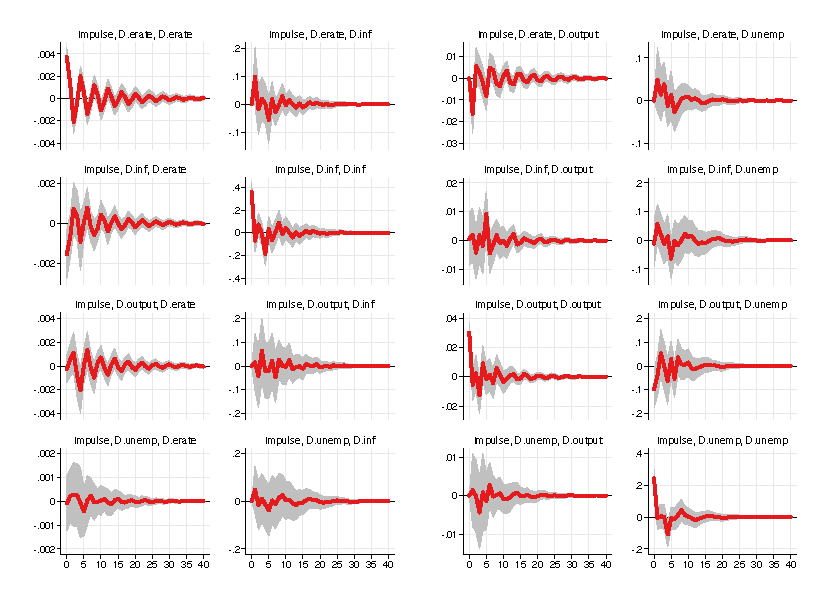
\includegraphics[width=1\linewidth]{../../empirical/Marcodata/Graphs/impulse_svar1}
		\begin{tablenotes}
		\footnotesize
		\item \textbf{Note:} This figure reports the impulse response of monetary policy shocks through the SVAR model on inflation, output, the exchange rate, and the unemployment rate over the horizon 1 to 42 quarters (a constant duration over the sample period 2010Q1–2021Q2) with four lags. All $y$-axis shows the percentage deviation from the pre-shock levels. The grey area shows 95\% bootstrapped confidence intervals for each impulse response.
		
	\end{tablenotes} 
\end{figure}

	%--------------------------------------------------------------------
\begin{figure}[H]
	\centering
	\caption{The impulse response to long-term monetary policy shocks}
	\label{fig:lsvar2}
	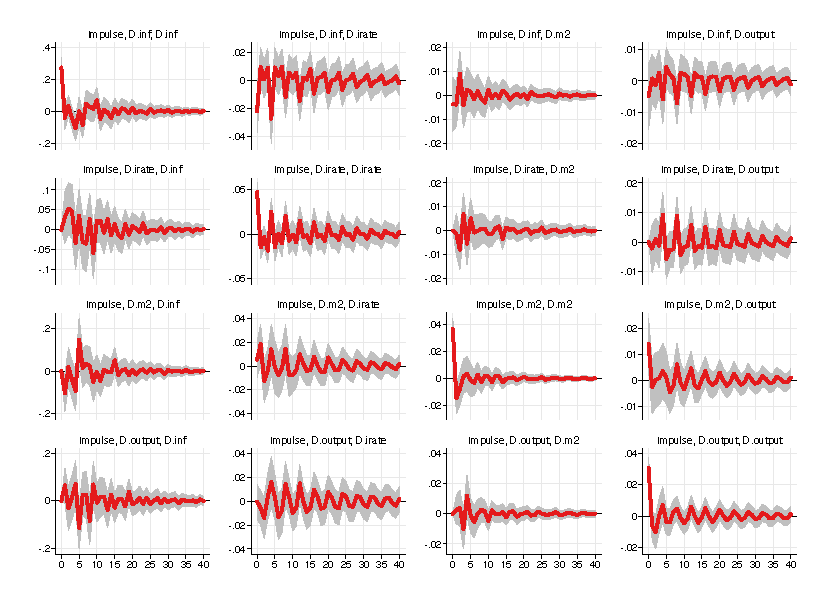
\includegraphics[width=1\linewidth]{../../empirical/Marcodata/Graphs/impulse_svar2}
	\begin{tablenotes}
		\footnotesize
		\item \textbf{Note:} This figure reports the impulse response of monetary policy shocks through the SVAR model on inflation, the interest rate, broad money and output over the horizon 1 to 42 quarters (a constant duration over the sample period 2010Q1–2021Q2) with four lags. All $y$-axis shows the percentage deviation from the pre-shock levels. The grey area shows 95\% bootstrapped confidence intervals for each impulse response.
		
	\end{tablenotes} 
\end{figure}
%--------------------------------------------------------------------

%-----------------------------------------------------------------------------------

	\subsection{Forecasting Errors Variance Decompositions }
	\begin{table}[H]
	\centering
	\caption{Forcasting errors variance decompositions from the SVAR model}
	\label{app:tabv1}
	\resizebox{.8\textwidth}{!}{%
		\begin{tabular}{@{}lccccc@{}}
			\hline \hline
			Variable                      & Horizon & Inflation & Output & Exchage rate & Unemployment \\ \hline
			\multirow{7}{*}{Inflation}  
			&1  & 1.0000 & 0.0004 & 0.1435 & 0.0019 \\
			&2  & 0.9173 & 0.0038 & 0.1480 & 0.0435 \\
			&3  & 0.9059 & 0.0171 & 0.1324 & 0.0470 \\
			&4  & 0.8790 & 0.0173 & 0.1328 & 0.0482 \\
			&8  & 0.8622 & 0.0745 & 0.1233 & 0.0779 \\
			&12 & 0.8552 & 0.0745 & 0.1234 & 0.0833 \\
			&40 & 0.8513 & 0.0776 & 0.1224 & 0.0864 \\ \hline
			
			\multirow{7}{*}{Output}       
			&1  & 0.0000 & 0.9996 & 0.0037 & 0.1364 \\
			&2  & 0.0016 & 0.7741 & 0.0186 & 0.1452 \\
			&3  & 0.0132 & 0.7451 & 0.0638 & 0.1736 \\
			&4  & 0.0390 & 0.7573 & 0.0872 & 0.1702 \\
			&8  & 0.0464 & 0.6742 & 0.2061 & 0.2105 \\
			&12 & 0.0498 & 0.6681 & 0.2183 & 0.2074 \\
			&40 & 0.0511 & 0.6555 & 0.2309 & 0.2069 \\ \hline
			
			\multirow{7}{*}{Exchage rate} 
			&1  & 0.0000 & 0.0000 & 0.8523 & 0.0000 \\
			&2  & 0.0655 & 0.2205 & 0.8303 & 0.0309 \\
			&3  & 0.0644 & 0.2362 & 0.7983 & 0.0320 \\
			&4  & 0.0652 & 0.2110 & 0.7723 & 0.0492 \\
			&8  & 0.0700 & 0.2339 & 0.6597 & 0.0482 \\
			&12 & 0.0707 & 0.2397 & 0.6483 & 0.0479 \\
			&40 & 0.0709 & 0.2491 & 0.6369 & 0.0483 \\ \hline
			
			\multirow{7}{*}{Unemployment} 
			&1  & 0.0000 & 0.0000 & 0.0005 & 0.8617 \\
			&2  & 0.0157 & 0.0016 & 0.0032 & 0.7804 \\
			&3  & 0.0165 & 0.0016 & 0.0054 & 0.7473 \\
			&4  & 0.0169 & 0.0144 & 0.0076 & 0.7324 \\
			&8  & 0.0214 & 0.0175 & 0.0109 & 0.6634 \\
			&12 & 0.0243 & 0.0176 & 0.0100 & 0.6614 \\
			&40 & 0.0268 & 0.0177 & 0.0099 & 0.6583 \\ \hline \hline
		\end{tabular}%
	}
	\begin{tablenotes}
	\footnotesize
	\item \textbf{Note:} This table reports the forecasting errors variance decomposition of the SVAR model through inflation, output, the exchange rate, and the unemployment rate over the horizon 1 to 40 quarters (a constant term over the 2010Q1--2021Q2 sample period) with 4 lags. Quantities in the table are percentages of the total factor variance. All entries are chi-square test statistics at dregress of freedom with an indicate significant at 1\%, 5\%, and 10\% levels, parentheses are $P$-values. 
	\end{tablenotes} 

\end{table}
	\begin{table}[H]
	\centering
	\caption{Forecasting errors variance decompositions from the SVAR model}
	\label{app:tabv2}
	\resizebox{.73\textwidth}{!}{%
		\begin{tabular}{@{}lccccc@{}}
			\hline \hline
			Variable                      & Horizon & Inflation & Output & M2 & Interest rate\\ \hline
			\multirow{7}{*}{Inflation}  
			&1  & 1.0000 & 0.0212 & 0.0100   & 0.174464 \\
			&2  & 0.8290 & 0.0208 & 0.0178   & 0.168138 \\
			&3  & 0.7955 & 0.0204 & 0.0613   & 0.152381 \\
			&4  & 0.7699 & 0.0255 & 0.0648   & 0.155954 \\
			&8  & 0.5572 & 0.0562 & 0.062701 & 0.231043 \\
			&12 & 0.5146 & 0.0817 & 0.068445 & 0.21545  \\
			&40 & 0.4930 & 0.1048 & 0.073112 & 0.218694 \\\hline
			
			\multirow{7}{*}{Output}       
			&1  & 0.0000 & 0.8135 & 0.0000   & 0.000091 \\
			&2  & 0.0450 & 0.8115 & 0.0045   & 0.009334 \\
			&3  & 0.0532 & 0.8245 & 0.0121   & 0.059227 \\
			&4  & 0.0520 & 0.8190 & 0.0632   & 0.05634  \\
			&8  & 0.1384 & 0.7151 & 0.132182 & 0.107807 \\
			&12 & 0.1767 & 0.6419 & 0.1429   & 0.131155 \\
			&40 & 0.1923 & 0.5781 & 0.1480   & 0.17266  \\\hline
			
			\multirow{7}{*}{M2} 
			&1  & 0.0000 & 0.1653 & 0.9900   & 0.009578 \\
			&2  & 0.1154 & 0.1640 & 0.9766   & 0.104275 \\
			&3  & 0.1128 & 0.1508 & 0.8906   & 0.135778 \\
			&4  & 0.1213 & 0.1502 & 0.8151   & 0.124358 \\
			&8  & 0.2468 & 0.1455 & 0.7298   & 0.113263 \\
			&12 & 0.2350 & 0.1518 & 0.7136   & 0.133484 \\
			&40 & 0.2348 & 0.1582 & 0.6958   & 0.138127 \\\hline
			
			\multirow{7}{*}{Interest rate} 
			&1  & 0.0000 & 0.0000 & 0.0000   & 0.815867 \\
			&2  & 0.0106 & 0.0037 & 0.0012   & 0.718252 \\
			&3  & 0.0385 & 0.0043 & 0.0361   & 0.652615 \\
			&4  & 0.0567 & 0.0053 & 0.0569   & 0.663348 \\
			&8  & 0.0576 & 0.0832 & 0.0753   & 0.547887 \\
			&12 & 0.0737 & 0.1246 & 0.0751   & 0.519912 \\
			&40 & 0.0798 & 0.1589 & 0.0831   & 0.470519 \\ \hline \hline
		\end{tabular}%
	}
	\begin{tablenotes}
	\footnotesize
	\item \textbf{Note:} This table reports the forecasting errors variance decomposition of the SVAR model through inflation, output, the broad money, and the interest rate over the horizon 1 to 40 quarters (a constant term over the 2010Q1--2021Q2 sample period) with 4 lags. Quantities in the table are percentages of the total factor variance. All entries are chi-square test statistics at dregress of freedom with an indicate significant at 1\%, 5\%, and 10\%  levels, parentheses are $P$-values. 
	\end{tablenotes} 
\end{table}


\begin{table}[]
	\begin{tabular}{lllll}
		
		
		
		
		
		
		
	\end{tabular}
\end{table}
	


	\subsection{Correlates of APCs and Exposures}
	This section is the supplementation of the correlation of APCs and their exposures that are presented in section \ref{sec:cova}. In other words, its perspectives on the empirical dives of my main error measurements through the monetary policy channels analysis.  
	
	\subsubsection{The Role of the Head of Household Age}	
	
	This section examines the distribution of exposures and APC by the head of household in each survey.  I divide the population into eight equally-sized age bins. The approach allows me to assess life-cycle dynamics and helps to visualize clearly the relative strengths and weaknesses of the CSES survey. 
	\vspace{1em}
	
	\noindent\textbf{Exposure Measures.} Figure \ref{fig:a33} presents the median value of $URE, NNP$ and gross income in each age bin normalized by average consumption in the three surveys. Average $URE$ (the orange line in the first row of graphs) is increasing in age across all three surveys, with a pattern of decline after retirement in the 2014 CSES data. In terms of magnitudes, average $URE$ is always positive in the 2014 CSES data, while in the 2017 and 2019/2020 CSES survey average $URE$ are negative for most working-age households, especially the head of household with age between 37 to 57. 
	
	Regrading net nominal positions that show in the second row of graphs report the life-cycle pattern in 2019/2020 is positive increasing in age. By contrast, the 2014 and 2017 datasets report $NNP$ unstable and negative with a minimum around age 45. In particular, in the 2017 CSES data, nominal liabilities are rising in age for young households and then start to decline steadily after age 42, while nominal assets are also declining for households age above 42.     
	\vspace{1em}
	
	\noindent\textbf{APC.} As shown in Figure \ref{fig:a33}, the fourth row reports the head of household age bins and average propensities to consume in all three surveys. Overall, there is a declining $APC$ in the old household for all three datasets. Interestingly, all three surveys suggest a rise $APC$ around middle age. The results appear that age is indeed a driver of the negative between $APC$ and exposure measures. 
	
	
		%-----------------------------------------------------------------------------------
		\begin{figure}
			\caption{Exposure measures by the head of household age bins in all three survey}
			\label{fig:a33}
			\begin{subfigure}{.33\textwidth}
				\centering
				\caption*{Panel A: CSES 2014}
				\label{fig:sub-first}
				\includegraphics[width=1\linewidth]{../../empirical/CSES2014/Appendix/Graphs/figc23_URE_agehead} 
				\vspace{-2.5em}
				\newline \centering{Age}
				
			\end{subfigure}
			\begin{subfigure}{.33\textwidth}
				\centering
				\caption*{Panel B: CSES 2017}
				\label{fig:sub-second}
				\includegraphics[width=1\linewidth]{../../empirical/CSES2017/Appendix/Graphs/figc23_URE_agehead} 
				\vspace{-2.5em}
				\newline \centering{Age}
				
			\end{subfigure}
			\begin{subfigure}{.33\textwidth}
				\centering
				\caption*{Panel C: CSES 2019}
				\label{fig:sub-first}
				
				\includegraphics[width=1\linewidth]{../../empirical/CSES2019/Appendix/Graphs/figc23_URE_agehead} 
				\vspace{-2.5em}
				\newline \centering{Age}
				
			\end{subfigure}
			
			\includegraphics[width=1\linewidth]{../../empirical/CSES2019/Appendix/Graphs/line_1} \vspace{-3em}
			\newline
			
			\begin{subfigure}{.33\textwidth}
				\centering
				\includegraphics[width=1\linewidth]{../../empirical/CSES2014/Appendix/Graphs/figc23_NNP_agehead} 
				\vspace{-2.5em}
				\newline \centering{Age}
			\end{subfigure}
			\begin{subfigure}{.33\textwidth}
				\centering
				\includegraphics[width=1\linewidth]{../../empirical/CSES2017/Appendix/Graphs/figc23_NNP_agehead} 
				\vspace{-2.5em}
				\newline \centering{Age}
			\end{subfigure}
			\begin{subfigure}{.33\textwidth}
				\centering
				\includegraphics[width=1\linewidth]{../../empirical/CSES2019/Appendix/Graphs/figc23_NNP_agehead} 
				\vspace{-2.5em}
				\newline \centering{Age}
			\end{subfigure}
			
			\includegraphics[width=1\linewidth]{../../empirical/CSES2019/Appendix/Graphs/line_2} 
			\vspace{-2.7em}
			\newline
			
			\begin{subfigure}{.33\textwidth}
				\centering
				\includegraphics[width=1\linewidth]{../../empirical/CSES2014/Appendix/Graphs/figc23_INC_agehead} 
				\vspace{-2.5em}
				\newline \centering{Age}
			\end{subfigure}
			\begin{subfigure}{.33\textwidth}
				\centering
				\includegraphics[width=1\linewidth]{../../empirical/CSES2017/Appendix/Graphs/figc23_INC_agehead} 
				\vspace{-2.5em}
				\newline \centering{Age}
			\end{subfigure}
			\begin{subfigure}{.33\textwidth}
				\centering
				\includegraphics[width=1\linewidth]{../../empirical/CSES2019/Appendix/Graphs/figc23_INC_agehead} 
				\vspace{-2.5em}
				\newline \centering{Age}
			\end{subfigure}
			
			\vspace{0em}
			\newline
			
			\begin{subfigure}{.33\textwidth}
				\centering
				\includegraphics[width=1\linewidth]{../../empirical/CSES2014/Appendix/Graphs/figc23_APC_agehead} 
				\vspace{-2.5em}
				\newline \centering{Age}
			\end{subfigure}
			\begin{subfigure}{.33\textwidth}
				\centering
				\includegraphics[width=1\linewidth]{../../empirical/CSES2017/Appendix/Graphs/figc23_APC_agehead} 
				\vspace{-2.5em}
				\newline \centering{Age}
			\end{subfigure}
			\begin{subfigure}{.33\textwidth}
				\centering
				\includegraphics[width=1\linewidth]{../../empirical/CSES2019/Appendix/Graphs/figc23_APC_agehead} 
				\vspace{-2.5em}
				\newline \centering{Age}
				
			\end{subfigure}
			
			
			\begin{tablenotes}
				\footnotesize
				\item \textbf{Note:} The figure plots all three exposure measures and estimated $APCs$ by age in all three surveys. Households are grouped by 8 equally-sized bins. The $x$-axis reports the average age in each group and the $y$-axis reports mean exposure as well as estimated $APC$ in each bin.
				
			\end{tablenotes} 
		\end{figure}
%-----------------------------------------------------------------------------------	

		\subsubsection{The Role of Household Income}	
		Figure \ref{fig:a34} examines the distribution of $URE$ and $NNP$ ($y$-axis) in all three datasets when the population is grouped into eight income bins. Median $URE$ is increasing in income, especially in the 2017 and 2019/2020 data. The increase of $URE$ is seen too much for households with the top income. At the same time, net nominal position patterns are the same tendency in the 2017 and 2019/2020 data. Households tend to raise nominal assets and nominal liabilities. 
		
		
		
		\begin{figure}
			\caption{URE and NNP components by income bins in all three surveys}
			\label{fig:a34}
			\begin{subfigure}{.33\textwidth}
				\centering
				\caption*{Panel A: CSES 2014}
				\label{fig:sub-first}
				\includegraphics[width=1\linewidth]{../../empirical/CSES2014/Appendix/Graphs/figc23_URE_NINC} 
				\vspace{-2.5em}
				\newline \centering{Normalized Gross Income}
				
			\end{subfigure}
			\begin{subfigure}{.33\textwidth}
				\centering
				\caption*{Panel B: CSES 2017}
				\label{fig:sub-second}
				\includegraphics[width=1\linewidth]{../../empirical/CSES2017/Appendix/Graphs/figc23_URE_NINC} 
				\vspace{-2.5em}
				\newline \centering{Normalized Gross Income}
				
			\end{subfigure}
			\begin{subfigure}{.33\textwidth}
				\centering
				\caption*{Panel C: CSES 2019}
				\label{fig:sub-first}
				
				\includegraphics[width=1\linewidth]{../../empirical/CSES2019/Appendix/Graphs/figc23_URE_NINC} 
				\vspace{-2.5em}
				\newline \centering{Normalized Gross Income}
				
			\end{subfigure}
			
			\includegraphics[width=1\linewidth]{../../empirical/CSES2019/Appendix/Graphs/line_1} \vspace{-3em}
			\newline
			
			\begin{subfigure}{.33\textwidth}
				\centering
				\includegraphics[width=1\linewidth]{../../empirical/CSES2014/Appendix/Graphs/figc23_NNP_NINC} 
				\vspace{-2.5em}
				\newline \centering{Normalized Gross Income}
			\end{subfigure}
			\begin{subfigure}{.33\textwidth}
				\centering
				\includegraphics[width=1\linewidth]{../../empirical/CSES2017/Appendix/Graphs/figc23_NNP_NINC} 
				\vspace{-2.5em}
				\newline \centering{Normalized Gross Income}
			\end{subfigure}
			\begin{subfigure}{.33\textwidth}
				\centering
				\includegraphics[width=1\linewidth]{../../empirical/CSES2019/Appendix/Graphs/figc23_NNP_NINC} 
				\vspace{-2.5em}
				\newline \centering{Normalized Gross Income}
			\end{subfigure}
			
			\includegraphics[width=1\linewidth]{../../empirical/CSES2019/Appendix/Graphs/line_2} 
			\vspace{-2.7em}
			\newline

			\begin{tablenotes}
				\footnotesize
				\item \textbf{Note:} The figure presents normalized $URE$ and normalized $NNP$, and estimated $APCs$ by income in all three surveys. Households are grouped by 8 equally-sized bins of gross income. The $x$-axis represents the average age in each group and the $y$-axis reports mean exposure as well as estimated $APC$ in each bin. 
				
			\end{tablenotes} 
		\end{figure}
		
		
		
		%-----------------------------------------------------------------------------------
		
		
%-----------------------------------------------------------------------------------
\subsubsection{A General Covariance Decomposition}
In part, I present a covariance decomposition that projected observables on a single covariate of CSES 2014--2019/2020. This approach can, of course, be generalized to include any number of covariates. Specifically, age groups, gender of head of household, marital status, year of education, household size, unemployed and household demographic. The procedure is in two steps: first, I run an OLS regression: 


\begin{align*}
	APC_{i} 	&= (\beta^m)' Z_{i} + \epsilon_{i}^m\\
	URE_{i} 	&= (\beta^u)' Z_{i} + \epsilon_{i}^u
\end{align*}
where $Z_{i} = (1, Z_{i1}, \cdots, Z_{iJ}})'$ is now a vector of covariates. Then, we recover fitted values
\begin{align*}
\widehat{APC}_{i}	&= (\widehat{\beta}_{m})' Z_{i}\\
\widehat{URE}_{i}	&= (\widehat{\beta}_{u})' Z_{i}
\end{align*}
and residual $\widehat{\epsilon_{i}^{m}}, \widehat{\epsilon_{i}^{u}}$. The law of total covariance can now be expressed as 

\begin{equation}
\mathrm{Cov}(APC_{i},URE_{i}) = \mathrm{Cov}(\widehat{APC_{i}},\widehat{URE_{i}}) + \mathrm{Cov}(\widehat{\epsilon_{i}^{m}},\widehat{\epsilon_{i}^{u}})
\end{equation}
The first term gives the component of explained covariance and the second the component of unexplained covariance. The explained paart of the covariance can be further decomposed as 
\begin{equation}\label{app:m2}
\mathrm{Cov}(\widehat{APC_{i}},\widehat{URE_{i}}) = \mathrm{Cov}(\sum_{j=1}^{J}\widehat{\beta_{j}^{m}}Z_{ij},\sum_{k=1}^{J}\widehat{\beta_{k}^{m}}Z_{ik}) = \sum_{j=1}^{J}\sum_{k=1}^{J}\widehat{\beta_{j}^{m}}\widehat{\beta_{k}^{m}}\mathrm{Cov}(Z_{ij},Z_{ik})
\end{equation}
Of course, the share of explained covariance is attributed to one particular covariate through this procedure on which other covariates are included in $Z_{i}$. 

\vspace{1em}
\noindent \textbf{Implementation: } Tables \ref{app:tc1}--\ref{tab:app13} report the full matrix described by equation (\ref{app:m2}) for each of my three main covariances $\mathcal{E}_{R}, \mathcal{E}_{P}$, and $\mathcal{E}_{Y}$ in three datasets, when all covariates from table \ref{tab:m6} are included simultaneously.

	\input{../../empirical/CSES2014/Appendix/Tables/tablec7.tex}    
	
	\input{../../empirical/CSES2017/Appendix/Tables/tablec7.tex}    

	
	\input{../../empirical/CSES2019/Appendix/Tables/tablec7.tex}    

%--------------------------------------------------------------------
\clearpage
\subsection{Gini Coefficient and Percentile Ratio}
\subsubsection{Household Income Inequality}
\begin{table}[H]
	\centering
	\caption{Forcasting errors variance decompositions from the SVAR model}
	\label{app:tabv1}
	\resizebox{.8\textwidth}{!}{%
		\begin{tabular}{@{}lccccc@{}}
			\hline \hline
			Variable                      & Horizon & Inflation & Output & Exchage rate & Unemployment \\ \hline
			\multirow{7}{*}{Inflation}  
			&1  & 1.0000 & 0.0004 & 0.1435 & 0.0019 \\
			&2  & 0.9173 & 0.0038 & 0.1480 & 0.0435 \\
			&3  & 0.9059 & 0.0171 & 0.1324 & 0.0470 \\
			&4  & 0.8790 & 0.0173 & 0.1328 & 0.0482 \\
			&8  & 0.8622 & 0.0745 & 0.1233 & 0.0779 \\
			&12 & 0.8552 & 0.0745 & 0.1234 & 0.0833 \\
			&40 & 0.8513 & 0.0776 & 0.1224 & 0.0864 \\ \hline
			
			\multirow{7}{*}{Output}       
			&1  & 0.0000 & 0.9996 & 0.0037 & 0.1364 \\
			&2  & 0.0016 & 0.7741 & 0.0186 & 0.1452 \\
			&3  & 0.0132 & 0.7451 & 0.0638 & 0.1736 \\
			&4  & 0.0390 & 0.7573 & 0.0872 & 0.1702 \\
			&8  & 0.0464 & 0.6742 & 0.2061 & 0.2105 \\
			&12 & 0.0498 & 0.6681 & 0.2183 & 0.2074 \\
			&40 & 0.0511 & 0.6555 & 0.2309 & 0.2069 \\ \hline
			
			\multirow{7}{*}{Exchage rate} 
			&1  & 0.0000 & 0.0000 & 0.8523 & 0.0000 \\
			&2  & 0.0655 & 0.2205 & 0.8303 & 0.0309 \\
			&3  & 0.0644 & 0.2362 & 0.7983 & 0.0320 \\
			&4  & 0.0652 & 0.2110 & 0.7723 & 0.0492 \\
			&8  & 0.0700 & 0.2339 & 0.6597 & 0.0482 \\
			&12 & 0.0707 & 0.2397 & 0.6483 & 0.0479 \\
			&40 & 0.0709 & 0.2491 & 0.6369 & 0.0483 \\ \hline
			
			\multirow{7}{*}{Unemployment} 
			&1  & 0.0000 & 0.0000 & 0.0005 & 0.8617 \\
			&2  & 0.0157 & 0.0016 & 0.0032 & 0.7804 \\
			&3  & 0.0165 & 0.0016 & 0.0054 & 0.7473 \\
			&4  & 0.0169 & 0.0144 & 0.0076 & 0.7324 \\
			&8  & 0.0214 & 0.0175 & 0.0109 & 0.6634 \\
			&12 & 0.0243 & 0.0176 & 0.0100 & 0.6614 \\
			&40 & 0.0268 & 0.0177 & 0.0099 & 0.6583 \\ \hline \hline
		\end{tabular}%
	}
	\begin{tablenotes}
	\footnotesize
	\item \textbf{Note:} This table reports the forecasting errors variance decomposition of the SVAR model through inflation, output, the exchange rate, and the unemployment rate over the horizon 1 to 40 quarters (a constant term over the 2010Q1--2021Q2 sample period) with 4 lags. Quantities in the table are percentages of the total factor variance. All entries are chi-square test statistics at dregress of freedom with an indicate significant at 1\%, 5\%, and 10\% levels, parentheses are $P$-values. 
	\end{tablenotes} 

\end{table}
\subsubsection{Household Consumption Inequality}
\begin{table}[H]
	\centering
	\caption{Forecasting errors variance decompositions from the SVAR model}
	\label{app:tabv2}
	\resizebox{.73\textwidth}{!}{%
		\begin{tabular}{@{}lccccc@{}}
			\hline \hline
			Variable                      & Horizon & Inflation & Output & M2 & Interest rate\\ \hline
			\multirow{7}{*}{Inflation}  
			&1  & 1.0000 & 0.0212 & 0.0100   & 0.174464 \\
			&2  & 0.8290 & 0.0208 & 0.0178   & 0.168138 \\
			&3  & 0.7955 & 0.0204 & 0.0613   & 0.152381 \\
			&4  & 0.7699 & 0.0255 & 0.0648   & 0.155954 \\
			&8  & 0.5572 & 0.0562 & 0.062701 & 0.231043 \\
			&12 & 0.5146 & 0.0817 & 0.068445 & 0.21545  \\
			&40 & 0.4930 & 0.1048 & 0.073112 & 0.218694 \\\hline
			
			\multirow{7}{*}{Output}       
			&1  & 0.0000 & 0.8135 & 0.0000   & 0.000091 \\
			&2  & 0.0450 & 0.8115 & 0.0045   & 0.009334 \\
			&3  & 0.0532 & 0.8245 & 0.0121   & 0.059227 \\
			&4  & 0.0520 & 0.8190 & 0.0632   & 0.05634  \\
			&8  & 0.1384 & 0.7151 & 0.132182 & 0.107807 \\
			&12 & 0.1767 & 0.6419 & 0.1429   & 0.131155 \\
			&40 & 0.1923 & 0.5781 & 0.1480   & 0.17266  \\\hline
			
			\multirow{7}{*}{M2} 
			&1  & 0.0000 & 0.1653 & 0.9900   & 0.009578 \\
			&2  & 0.1154 & 0.1640 & 0.9766   & 0.104275 \\
			&3  & 0.1128 & 0.1508 & 0.8906   & 0.135778 \\
			&4  & 0.1213 & 0.1502 & 0.8151   & 0.124358 \\
			&8  & 0.2468 & 0.1455 & 0.7298   & 0.113263 \\
			&12 & 0.2350 & 0.1518 & 0.7136   & 0.133484 \\
			&40 & 0.2348 & 0.1582 & 0.6958   & 0.138127 \\\hline
			
			\multirow{7}{*}{Interest rate} 
			&1  & 0.0000 & 0.0000 & 0.0000   & 0.815867 \\
			&2  & 0.0106 & 0.0037 & 0.0012   & 0.718252 \\
			&3  & 0.0385 & 0.0043 & 0.0361   & 0.652615 \\
			&4  & 0.0567 & 0.0053 & 0.0569   & 0.663348 \\
			&8  & 0.0576 & 0.0832 & 0.0753   & 0.547887 \\
			&12 & 0.0737 & 0.1246 & 0.0751   & 0.519912 \\
			&40 & 0.0798 & 0.1589 & 0.0831   & 0.470519 \\ \hline \hline
		\end{tabular}%
	}
	\begin{tablenotes}
	\footnotesize
	\item \textbf{Note:} This table reports the forecasting errors variance decomposition of the SVAR model through inflation, output, the broad money, and the interest rate over the horizon 1 to 40 quarters (a constant term over the 2010Q1--2021Q2 sample period) with 4 lags. Quantities in the table are percentages of the total factor variance. All entries are chi-square test statistics at dregress of freedom with an indicate significant at 1\%, 5\%, and 10\%  levels, parentheses are $P$-values. 
	\end{tablenotes} 
\end{table}


\begin{table}[]
	\begin{tabular}{lllll}
		
		
		
		
		
		
		
	\end{tabular}
\end{table}
\subsubsection{Household Assets Inequality}
\input{../../empirical/table_a3.tex}    
\subsubsection{Household Liabilities Inequality}
\input{../../empirical/table_a4.tex}    



%--------------------------------------------------------------------
\clearpage


\subsubsection{Income Inequality through Education Group}

In this section, I provide additional information on household income distribution through the Gini coefficient of income share by a group of the head family education. I diversified five education groups, primary school, secondary school, high school, junior college and bachelor's degree. Figures \ref{fig:app18}--\ref{fig:app20} show the Gini index of income share by years of schooling groups. It is interesting to note that the index of income inequality among households who received bachelor's degree is very low than others, with around 0.472 in 2014 to 0.331 in 2019/2020. 
%--------------------------------------------------------------------
\begin{figure}[H]
	\centering
	\caption{Gini index of household income by education group in 2014}
	\label{fig:app18}
	\includegraphics[width=1\linewidth]{../../empirical/CSES2014/Appendix/Graphs/percentiles_inc_educ}

\end{figure}
%--------------------------------------------------------------------

%--------------------------------------------------------------------
\begin{figure}
	\centering
		\caption{Gini index of household income by education group in 2017}
	\label{}
	\vspace{-1em}
	\includegraphics[width=1\linewidth]{../../empirical/CSES2017/Appendix/Graphs/percentiles_inc_educ}

\end{figure}
%--------------------------------------------------------------------

%--------------------------------------------------------------------
\begin{figure}
	\centering
		\caption{Gini index of household income by education group in 2019/2020}
	\label{fig:app20}
		\vspace{-1em}
	\includegraphics[width=1\linewidth]{../../empirical/CSES2019/Appendix/Graphs/percentiles_inc_educ}

\end{figure}
%--------------------------------------------------------------------


\subsection{Median Income by Household Structure}
%-----------------------------------------------------------------------------------
\begin{figure}[H]
	\caption{Median household income by type}
	\label{fig:app21}
	\begin{subfigure}[b]{0.33\linewidth}
		\caption*{Panel A: CSES 2014} \vspace{-.5em}
		\label{fig:3a}
		\includegraphics[width=1\linewidth]{../../empirical/CSES2014/Appendix/Graphs/inc_earner} 
		\vspace{-2.5em}
		\newline \centering{Number of Earners}
		\includegraphics[width=1\linewidth]{../../empirical/CSES2014/Appendix/Graphs/inc_educhead} 
		\vspace{-2.5em}
		\newline \centering{Years of Education}
		\includegraphics[width=1\linewidth]{../../empirical/CSES2014/Appendix/Graphs/inc_nmember} 
		\vspace{-2.5em}
		\newline \centering{Household's Member}
		\includegraphics[width=1\linewidth]{../../empirical/CSES2014/Appendix/Graphs/inc_region} 
		\vspace{-2.5em}
		\newline \centering{Regions}
	\end{subfigure}%
	\hfil
	\begin{subfigure}[b]{0.33\linewidth}
		\caption*{Panel B: CSES 2017} \vspace{-.5em}
		\label{fig:3b}
		\includegraphics[width=1\linewidth]{../../empirical/CSES2017/Appendix/Graphs/inc_earner} 
		\vspace{-2.5em}
		\newline \centering{Number of Earners}
		\includegraphics[width=1\linewidth]{../../empirical/CSES2017/Appendix/Graphs/inc_educhead} 
		\vspace{-2.5em}
		\newline \centering{Years of Education}
		\includegraphics[width=1\linewidth]{../../empirical/CSES2017/Appendix/Graphs/inc_nmember} 
		\vspace{-2.5em}
		\newline \centering{Household's Member}
		\includegraphics[width=1\linewidth]{../../empirical/CSES2017/Appendix/Graphs/inc_region} 
		\vspace{-2.5em}
		\newline \centering{Regions}
	\end{subfigure}
	\hfil
	\begin{subfigure}[b]{0.33\linewidth}
		\caption*{Panel C: CSES 2019} \vspace{-.5em}
		\label{fig:3c}
		\includegraphics[width=1\linewidth]{../../empirical/CSES2019/Appendix/Graphs/inc_earner} 
		\vspace{-2.5em}
		\newline \centering{Number of Earners}
		\includegraphics[width=1\linewidth]{../../empirical/CSES2019/Appendix/Graphs/inc_educhead} 
		\vspace{-2.5em}
		\newline \centering{Years of Education}
		\includegraphics[width=1\linewidth]{../../empirical/CSES2019/Appendix/Graphs/inc_nmember} 
		\vspace{-2.5em}
		\newline \centering{Household's Member}
		\includegraphics[width=1\linewidth]{../../empirical/CSES2019/Appendix/Graphs/inc_region} 
		\vspace{-2.5em}
		\newline \centering{Regions}
	\end{subfigure}
	
	\begin{tablenotes}
		\footnotesize
		\item \textbf{Note:} These figures show the average household income by group: earner numbers, school years, family members, and family regions. The $y$ axis is the value of income in US dollars in 1,000. 
		
	\end{tablenotes} 
\end{figure}



\begin{figure}[H]
	\caption{Scatter plot of the logarithm of household income ($log(Y_{i})$)}
	
	
	\label{fig:3}
	\begin{subfigure}[b]{0.33\linewidth}
		\caption*{Panel A: CSES 2014} \vspace{-.5em}
		\label{fig:3a}
		\includegraphics[width=1\linewidth]{../../empirical/CSES2014/Appendix/Graphs/ln_y_ln_c} 
		\vspace{-2.5em}
		\newline \centering{$log(C_{i})$}
		\includegraphics[width=1\linewidth]{../../empirical/CSES2014/Appendix/Graphs/ln_y_ln_hwork} 
		\vspace{-2.5em}
		\newline \centering{$log(W_{t})$}
	\end{subfigure}%
	\hfil
	\begin{subfigure}[b]{0.33\linewidth}
		\caption*{Panel B: CSES 2017} \vspace{-.5em}
		\label{fig:3b}
		\includegraphics[width=1\linewidth]{../../empirical/CSES2017/Appendix/Graphs/ln_y_ln_c} 
		\vspace{-2.5em}
		\newline \centering{$log(C_{i})$}
		\includegraphics[width=1\linewidth]{../../empirical/CSES2017/Appendix/Graphs/ln_y_ln_hwork}
		\vspace{-2.5em}
		\newline \centering{$log(W_{t})$}
	\end{subfigure}
	\hfil
	\begin{subfigure}[b]{0.33\linewidth}
		\caption*{Panel C: CSES 2019} \vspace{-.5em}
		\label{fig:3c}
		\includegraphics[width=1\linewidth]{../../empirical/CSES2019/Appendix/Graphs/ln_y_ln_c} 
		\vspace{-2.5em}
		\newline \centering{$log(C_{i})$}
		\includegraphics[width=1\linewidth]{../../empirical/CSES2019/Appendix/Graphs/ln_y_ln_hwork} 
		\vspace{-2.5em}
		\newline \centering{$log(W_{t})$}
	\end{subfigure}
	\begin{tablenotes}
		\footnotesize
		\item \textbf{Note:} The figure reports a result of scatter plot of the logarithm of household income with the logarithm of consumption and total hours of worked. The $x$-axis represents the value of log consumption in \$1,000 and the value of log total hours of worked. The $y$-axis is the log income in \$1,000. Panel A reports the 2014 CSES data, Panel B is the 2017 CSES data and Panel C is the 2019/2020 CSES data.  
		
	\end{tablenotes} 
	
\end{figure}

%-----------------------------------------------------------------------------------


\subsection{Median Consumption by Household Structure}
%-----------------------------------------------------------------------------------
\begin{figure}[H]
	\caption{Average household consumption by type}
	\label{fig:3}
	\begin{subfigure}[b]{0.33\linewidth}
		\caption*{Panel A: CSES 2014} \vspace{-.5em}
		\label{fig:3a}
		\includegraphics[width=1\linewidth]{../../empirical/CSES2014/Appendix/Graphs/cons_earner} 
		\vspace{-2.5em}
		\newline \centering{Number of Earners}
		\includegraphics[width=1\linewidth]{../../empirical/CSES2014/Appendix/Graphs/cons_educhead} 
		\vspace{-2.5em}
		\newline \centering{Years of Education}
		\includegraphics[width=1\linewidth]{../../empirical/CSES2014/Appendix/Graphs/cons_nmember} 
		\vspace{-2.5em}
		\newline \centering{Household's Member}
		\includegraphics[width=1\linewidth]{../../empirical/CSES2014/Appendix/Graphs/cons_region} 
		\vspace{-2.5em}
		\newline \centering{Regions}
	\end{subfigure}%
	\hfil
	\begin{subfigure}[b]{0.33\linewidth}
		\caption*{Panel B: CSES 2017} \vspace{-.5em}
		\label{fig:3b}
		\includegraphics[width=1\linewidth]{../../empirical/CSES2017/Appendix/Graphs/cons_earner} 
		\vspace{-2.5em}
		\newline \centering{Number of Earners}
		\includegraphics[width=1\linewidth]{../../empirical/CSES2017/Appendix/Graphs/cons_educhead} 
		\vspace{-2.5em}
		\newline \centering{Years of Education}
		\includegraphics[width=1\linewidth]{../../empirical/CSES2017/Appendix/Graphs/cons_nmember} 
		\vspace{-2.5em}
		\newline \centering{Household's Member}
		\includegraphics[width=1\linewidth]{../../empirical/CSES2017/Appendix/Graphs/cons_region} 
		\vspace{-2.5em}
		\newline \centering{Regions}
	\end{subfigure}
	\hfil
	\begin{subfigure}[b]{0.33\linewidth}
		\caption*{Panel C: CSES 2019} \vspace{-.5em}
		\label{fig:3c}
		\includegraphics[width=1\linewidth]{../../empirical/CSES2019/Appendix/Graphs/cons_earner} 
		\vspace{-2.5em}
		\newline \centering{Number of Earners}
		\includegraphics[width=1\linewidth]{../../empirical/CSES2019/Appendix/Graphs/cons_educhead} 
		\vspace{-2.5em}
		\newline \centering{Years of Education}
		\includegraphics[width=1\linewidth]{../../empirical/CSES2019/Appendix/Graphs/cons_nmember} 
		\vspace{-2.5em}
		\newline \centering{Household's Member}
		\includegraphics[width=1\linewidth]{../../empirical/CSES2019/Appendix/Graphs/cons_region} 
		\vspace{-2.5em}
		\newline \centering{Regions}
	\end{subfigure}
	
		\begin{tablenotes}
		\footnotesize
		\item \textbf{Note:} These figures show the average household expenditure by group: earner numbers, school years, family members, and family regions. The $y$ axis is the value of spending in US dollars in 1,000. 
		
	\end{tablenotes} 
\end{figure}

%-----------------------------------------------------------------------------------

%-----------------------------------------------------------------------------------

\subsection{Household Wealth through Education, Age and Region}
\vspace{-1.2em}
%-----------------------------------------------------------------------------------
\begin{figure}[H]
	\caption{Sex and education of the head of household}
	\label{fig:3}
	\vspace{-.8em}
	\begin{subfigure}[b]{0.33\linewidth}
		\caption*{Panel A: CSES 2014} \vspace{-.5em}
		\label{fig:3a}
		\includegraphics[width=1\linewidth]{../../empirical/CSES2014/Appendix/Graphs/educ_y} 
		\vspace{-2.5em}
		\newline \centering{Household Income}
		\includegraphics[width=1\linewidth]{../../empirical/CSES2014/Appendix/Graphs/educ_cc} 	\vspace{-2.5em}
		\newline \centering{Household Consumption}
		\includegraphics[width=1\linewidth]{../../empirical/CSES2014/Appendix/Graphs/educ_asset} 
		\vspace{-2.5em}
		\newline \centering{Household Assets}
		\includegraphics[width=1\linewidth]{../../empirical/CSES2014/Appendix/Graphs/educ_liab} 
		\vspace{-2.5em}
		\newline \centering{Household Liabilities}
	\end{subfigure}%
	\hfil
	\begin{subfigure}[b]{0.33\linewidth}
		\caption*{Panel B: CSES 2017} \vspace{-.5em}
		\label{fig:3b}
		\includegraphics[width=1\linewidth]{../../empirical/CSES2017/Appendix/Graphs/educ_y}
		\vspace{-2.5em}
		\newline \centering{Household Income} 
		\includegraphics[width=1\linewidth]{../../empirical/CSES2017/Appendix/Graphs/educ_cc}
		\vspace{-2.5em}
		\newline \centering{Household Consumption} 
		\includegraphics[width=1\linewidth]{../../empirical/CSES2017/Appendix/Graphs/educ_asset} 
		\vspace{-2.5em}
		\newline \centering{Household Assets}
		\includegraphics[width=1\linewidth]{../../empirical/CSES2017/Appendix/Graphs/educ_liab} 
		\vspace{-2.5em}
		\newline \centering{Household Liabilities}
	\end{subfigure}
	\hfil
	\begin{subfigure}[b]{0.33\linewidth}
		\caption*{Panel C: CSES 2019} \vspace{-.5em}
		\label{fig:3c}
		\includegraphics[width=1\linewidth]{../../empirical/CSES2019/Appendix/Graphs/educ_y}
		\vspace{-2.5em}
		\newline \centering{Household Income} 
		\includegraphics[width=1\linewidth]{../../empirical/CSES2019/Appendix/Graphs/educ_cc}
		\vspace{-2.5em}
		\newline \centering{Household Consumption} 
		\includegraphics[width=1\linewidth]{../../empirical/CSES2019/Appendix/Graphs/educ_asset} 
		\vspace{-2.5em}
		\newline \centering{Household Assets}
		\includegraphics[width=1\linewidth]{../../empirical/CSES2019/Appendix/Graphs/educ_liab} 
		\vspace{-2.5em}
		\newline \centering{Household Liabilities}
	\end{subfigure}
		\includegraphics[width=1\linewidth]{../../empirical/CSES2019/Appendix/Graphs/line_3} 
	\begin{tablenotes}
		\footnotesize
		\item \textbf{Note:} These graphs show the gender of the head of household by years of education groups. The blue line represents years of schooling at the primary school, the green line is the secondary school, the light blue is the high school, the orange line is the junior college, and the red line is the undergraduate degree. Panel A reports the 2014 CSES data, Panel B is the 2017 CSES data and Panel C is the 2019/2020 CSES data. All $y$-axis represent the value of household income, consumption, assets and liabilities in \$1,000. It is the sum of all sources of wealth and spending in a family that must neglect the years of schooling of the head family. It is important to remember that all members of a household have different years of schooling. 
	\end{tablenotes} 
	
\end{figure}

%-----------------------------------------------------------------------------------
%-----------------------------------------------------------------------------------
\begin{figure}[H]
	\caption{Mean household assets by five main regions across the nation}
	\label{fig:3}
	\begin{subfigure}[b]{0.33\linewidth}
		\caption*{Panel A: CSES 2014} \vspace{-.5em}
		\label{fig:3a}
		\includegraphics[width=1\linewidth]{../../empirical/CSES2014/Appendix/Graphs/region_houseasset} 
		\vspace{-2.5em}
		\newline \centering{Housing Assets}
		\includegraphics[width=1\linewidth]{../../empirical/CSES2014/Appendix/Graphs/region_buildasset} 
		\vspace{-2.5em}
		\newline \centering{Building Assets}
		\includegraphics[width=1\linewidth]{../../empirical/CSES2014/Appendix/Graphs/region_landasset} 
		\vspace{-2.5em}
		\newline \centering{Land Assets}
		\includegraphics[width=1\linewidth]{../../empirical/CSES2014/Appendix/Graphs/region_dgoodsasset} 
		\vspace{-2.5em}
		\newline \centering{Durable Goods Assets}
	\end{subfigure}%
	\hfil
	\begin{subfigure}[b]{0.33\linewidth}
		\caption*{Panel B: CSES 2017} \vspace{-.5em}
		\label{fig:3b}
		\includegraphics[width=1\linewidth]{../../empirical/CSES2017/Appendix/Graphs/region_houseasset} 
		\vspace{-2.5em}
		\newline \centering{Housing Assets}
		\includegraphics[width=1\linewidth]{../../empirical/CSES2017/Appendix/Graphs/region_buildasset} 
		\vspace{-2.5em}
		\newline \centering{Building Assets}
		\includegraphics[width=1\linewidth]{../../empirical/CSES2017/Appendix/Graphs/region_landasset} 
		\vspace{-2.5em}
		\newline \centering{Land Assets}
		\includegraphics[width=1\linewidth]{../../empirical/CSES2017/Appendix/Graphs/region_dgoodsasset} 
		\vspace{-2.5em}
		\newline \centering{Durable Goods Assets}
	\end{subfigure}
	\hfil
	\begin{subfigure}[b]{0.33\linewidth}
		\caption*{Panel C: CSES 2019} \vspace{-.5em}
		\label{fig:3c}
		\includegraphics[width=1\linewidth]{../../empirical/CSES2019/Appendix/Graphs/region_houseasset} 
		\vspace{-2.5em}
		\newline \centering{Housing Assets}
		\includegraphics[width=1\linewidth]{../../empirical/CSES2019/Appendix/Graphs/region_buildasset} 
		\vspace{-2.5em}
		\newline \centering{Building Assets}
		\includegraphics[width=1\linewidth]{../../empirical/CSES2019/Appendix/Graphs/region_landasset} 
		\vspace{-2.5em}
		\newline \centering{Land Assets}
		\includegraphics[width=1\linewidth]{../../empirical/CSES2019/Appendix/Graphs/region_dgoodsasset} 
		\vspace{-2.5em}
		\newline \centering{Durable Goods Assets}
	\end{subfigure}
		\includegraphics[width=1\linewidth]{../../empirical/CSES2019/Appendix/Graphs/line_region} 
	
	\begin{tablenotes}
		\footnotesize
		\item \textbf{Note:} The graph plots the average household wealth by types of assets such as housing assets, building assets, land assets and durable goods assets in the different regions. Panel A reports the 2014 CSES data, Panel B is the 2017 CSES data and Panel C is the 2019/2020 CSES data. The red line is Phnom Penh, the blue is the central plains, the green is Tonle Sap, the purple is Coastal and the orange is Plateau and Mountains region. All $y$-axis represent the value of assets in \$1,000.
	\end{tablenotes} 
\end{figure}


%-----------------------------------------------------------------------------------
\begin{figure}
	\caption{Lorenz curve of household income, consumption and assets}
	\label{fig:fig}
	\begin{subfigure}{.33\textwidth}
		\centering
		\caption*{Panel A: CSES 2014}
		\label{fig:sub-first}
		\includegraphics[width=1\linewidth]{../../empirical/CSES2014/Appendix/Graphs/lorez_inc}
		
	\end{subfigure}
	\begin{subfigure}{.33\textwidth}
		\centering
		\caption*{Panel B: CSES 2017}
		\label{fig:sub-second}
		\includegraphics[width=1\linewidth]{../../empirical/CSES2017/Appendix/Graphs/lorez_inc}
		
	\end{subfigure}
	\begin{subfigure}{.33\textwidth}
		\centering
		\caption*{Panel C: CSES 2019}
		\label{fig:sub-first}
		\includegraphics[width=1\linewidth]{../../empirical/CSES2019/Appendix/Graphs/lorez_inc}
		
	\end{subfigure}
	\includegraphics[width=1\linewidth]{../../empirical/CSES2019/Appendix/Graphs/line_inc}
	\vspace{-3em}
	\newline
	
	\begin{subfigure}{.33\textwidth}
		\centering
		\includegraphics[width=1\linewidth]{../../empirical/CSES2014/Appendix/Graphs/lorez_con} 	
		
	\end{subfigure}
	\begin{subfigure}{.33\textwidth}
		\centering
		\includegraphics[width=1\linewidth]{../../empirical/CSES2014/Appendix/Graphs/lorez_con} 	
	\end{subfigure}
	\begin{subfigure}{.33\textwidth}
		\centering
		\includegraphics[width=1\linewidth]{../../empirical/CSES2014/Appendix/Graphs/lorez_con} 	
		
	\end{subfigure}
	\includegraphics[width=1\linewidth]{../../empirical/CSES2019/Appendix/Graphs/line_cons} \vspace{-3em}
	\newline
	
	\begin{subfigure}{.33\textwidth}
		\centering
		\includegraphics[width=1\linewidth]{../../empirical/CSES2014/Appendix/Graphs/lorez_ass} 		
		
	\end{subfigure}
	\begin{subfigure}{.33\textwidth}
		\centering
		\includegraphics[width=1\linewidth]{../../empirical/CSES2014/Appendix/Graphs/lorez_ass} 		
	\end{subfigure}
	\begin{subfigure}{.33\textwidth}
		\centering
		\includegraphics[width=1\linewidth]{../../empirical/CSES2014/Appendix/Graphs/lorez_ass} 		
	\end{subfigure}
	\includegraphics[width=1\linewidth]{../../empirical/CSES2019/Appendix/Graphs/line_ass} 		
	
	\begin{tablenotes}
		\footnotesize
		\item \textbf{Note:} These graphs represent the Lorenz curve of household wealth between 2014--2019/2020 by using the CSES dataset. The first row is the average household income by types of sources, including wages, business income, agricultural incomes, and other incomes. The second row reports the Lorenz curve of the median household expenditure in different factors such as foods, nonfoods, housing spending, and durable goods. The third row is the curve for household assets. The $x$-axis is the population percentage and the $y$-axis is the cumulative outcome proposition.  
		
	\end{tablenotes} 
\end{figure}


%-----------------------------------------------------------------------------------
\begin{figure}
	\caption{Average household income and consumption by age group}
	\label{fig:3}
	\begin{subfigure}[b]{0.33\linewidth}
		\caption*{Panel A: CSES 2014} \vspace{-.5em}
		\label{fig:3a}
		\includegraphics[width=1\linewidth]{../../empirical/CSES2014/Appendix/Graphs/inc_agejpbin} 
		\vspace{-2.5em}
		\newline \centering{Income and Age}
		\includegraphics[width=1\linewidth]{../../empirical/CSES2014/Appendix/Graphs/cons_agejpbin} 
		\vspace{-2.5em}
		\newline \centering{Consumption and Age}
	\end{subfigure}%
	\hfil
	\begin{subfigure}[b]{0.33\linewidth}
		\caption*{Panel B: CSES 2017} \vspace{-.5em}
		\label{fig:3b}
		\includegraphics[width=1\linewidth]{../../empirical/CSES2017/Appendix/Graphs/inc_agejpbin} 
		\vspace{-2.5em}
		\newline \centering{Income and Age}
		\includegraphics[width=1\linewidth]{../../empirical/CSES2017/Appendix/Graphs/cons_agejpbin} 
		\vspace{-2.5em}
		\newline \centering{Consumption and Age}
	\end{subfigure}
	\hfil
	\begin{subfigure}[b]{0.33\linewidth}
		\caption*{Panel C: CSES 2019} \vspace{-.5em}
		\label{fig:3c}
		\includegraphics[width=1\linewidth]{../../empirical/CSES2019/Appendix/Graphs/inc_agejpbin} 
		\vspace{-2.5em}
		\newline \centering{Income and Age}
		\includegraphics[width=1\linewidth]{../../empirical/CSES2019/Appendix/Graphs/cons_agejpbin} 
		\vspace{-2.5em}
		\newline \centering{Consumption and Age}
	\end{subfigure}
	
		\begin{tablenotes}
		\footnotesize
		\item \textbf{Note:} The figure represents the median household income and expenditure between 2014--2019/2020 by using the CSES dataset. The first row is the average household income by group of age. The second row reports the median household expenditure by group of age. All $y$-axis is the value of income and spending in US dollars in 1,000. 
	\end{tablenotes} 
\end{figure}

%-----------------------------------------------------------------------------------

%-----------------------------------------------------------------------------------

\subsection{The Interest Rate and Loans}\label{sec:appirate}
%-----------------------------------------------------------------------------------
\begin{figure}[H]
	\caption{The annual interest rate and monthly interest rate of household liabilities }
	\label{fig:appirate}
	\begin{subfigure}[b]{0.33\linewidth}
		\caption*{Panel A: CSES 2014} \vspace{-.5em}
		\includegraphics[width=1\linewidth]{../../empirical/CSES2014/Appendix/Graphs/irates} 
		\vspace{-2.5em}
		\newline \centering{Annual Interest Rate}
		
		\includegraphics[width=1\linewidth]{../../empirical/CSES2014/Appendix/Graphs/lmonth} 
		\vspace{-2.5em}
		\newline \centering{Monthly Interest Rate}
		
	\end{subfigure}%
	\hfil
	\begin{subfigure}[b]{0.33\linewidth}
		\caption*{Panel B: CSES 2017} \vspace{-.5em}
		\includegraphics[width=1\linewidth]{../../empirical/CSES2017/Appendix/Graphs/irates} 
		\vspace{-2.5em}
		\newline \centering{Annual Interest Rate}
		
		\includegraphics[width=1\linewidth]{../../empirical/CSES2017/Appendix/Graphs/lmonth}
		\vspace{-2.5em}
		\newline \centering{Monthly Interest Rate}
	\end{subfigure}
	\hfil
	\begin{subfigure}[b]{0.33\linewidth}
		\caption*{Panel C: CSES 2019} \vspace{-.5em}
		\includegraphics[width=1\linewidth]{../../empirical/CSES2019/Appendix/Graphs/irates} 
		\vspace{-2.5em}
		\newline \centering{Annual Interest Rate}
		
		\includegraphics[width=1\linewidth]{../../empirical/CSES2019/Appendix/Graphs/lmonth} 
		\vspace{-2.5em}
		\newline \centering{Monthly Interest Rate}
	\end{subfigure}
	\begin{tablenotes}
		\footnotesize
		\item \textbf{Note:} This figure reports the annual interest rate and monthly interest rate of household's loans in different regions. Panel A shows the interest rate of the 2014 CSES data, Panel B is the 2017 CSES data and Panel C presents the 2019/2020 CSES dataset. The first row is the annual rate and the second row is the monthly interest rate. The $y$-axis represents the percentage of interest rates.   
		
	\end{tablenotes} 
	
	
\end{figure}

%-----------------------------------------------------------------------------------

%-----------------------------------------------------------------------------------
\begin{figure}[H]
	\caption{The value of loans and their objectives}
	\label{fig:7}
	\begin{subfigure}[b]{0.33\linewidth}
		\caption*{Panel A: CSES 2014} \vspace{-.5em}
		\label{fig:3a}
		\includegraphics[width=1\linewidth]{../../empirical/CSES2014/Appendix/Graphs/histo_liab} 
	\end{subfigure}%
	\hfil
	\begin{subfigure}[b]{0.33\linewidth}
		\caption*{Panel B: CSES 2017} \vspace{-.5em}
		\label{fig:3b}
		\includegraphics[width=1\linewidth]{../../empirical/CSES2017/Appendix/Graphs/histo_liab} 
	\end{subfigure}
	\hfil
	\begin{subfigure}[b]{0.33\linewidth}
		\caption*{Panel C: CSES 2019} \vspace{-.5em}
		\label{fig:3c}
		\includegraphics[width=1\linewidth]{../../empirical/CSES2019/Appendix/Graphs/histo_liab} 
	\end{subfigure}
	\begin{tablenotes}
		\footnotesize
		\item \textbf{Note:} The figure shows the value of household liabilities by objective of loans and amount of values. The $y$-axis is the value of US dollar loans in 1000. All three graphs used sample weight and eliminated the low- and high-loan household at the percentile 1\%. I determine the purposes of a loan into four types: for production, consumption, repayment of other debts, and other purposes.    
	\end{tablenotes} 
	
\end{figure}

%-----------------------------------------------------------------------------------












%\clearpage	
%{\small
	%\bibliographystyle{jpe} % is refer to the Journal of Political Economy
	%\bibliographystyle{apecon}
	%\bibliographystyle{ier}
%	\bibliographystyle{aea}  % is refer to the American Economic Association
	%\bibliographystyle{ecca} % is refer to the Journal of Economica
%	\bibliography{References}
%}	
%--------------------------------------------------------------------

\end{document}
